\documentclass[11pt,letterpaper]{article}
%\documentclass[11pt,a4paper]{report}

\usepackage{tikz}
\usepackage{amssymb,amsmath,amsthm} 
\usepackage[margin=2cm]{geometry}
\usepackage{fancyhdr}
\usepackage{enumitem}
\usepackage[compact]{titlesec}
\usepackage{graphicx,ctable,booktabs,subcaption}

\usepackage{xparse,hyperref,parskip}

%\newcommand{\abs}[1]{\left|#1\right|}

\newcommand{\semester}{Spring 2022}
\newcommand{\due}{Thursday, April 7}


\pagestyle{fancy}
\lhead{ }
\chead{\footnotesize Math 3338\quad  Numerical Methods\quad  \semester}
\rhead{\footnotesize \thepage}
\setlength{\parindent}{0cm}
\setlist{noitemsep}



\newtheorem{theorem}{Theorem}

\input{defs.tex}

%Defines the problem environment with arguments Points and Solution gap
\input{problem_env.tex}


\newcommand{\shrug}[1][]{%
\begin{tikzpicture}[baseline,x=0.8\ht\strutbox,y=0.8\ht\strutbox,line width=0.125ex,#1]
\def\arm{(-2.5,0.95) to (-2,0.95) (-1.9,1) to (-1.5,0) (-1.35,0) to (-0.8,0)};
\draw \arm;
\draw[xscale=-1] \arm;
\def\headpart{(0.6,0) arc[start angle=-40, end angle=40,x radius=0.6,y radius=0.8]};
\draw \headpart;
\draw[xscale=-1] \headpart;
\def\eye{(-0.075,0.15) .. controls (0.02,0) .. (0.075,-0.15)};
\draw[shift={(-0.3,0.8)}] \eye;
\draw[shift={(0,0.85)}] \eye;
% draw mouth
\draw (-0.1,0.2) to [out=15,in=-100] (0.4,0.95); 
\end{tikzpicture}}



\begin{document}

\begin{center}
{\huge{\bf  Numerical Methods}} \\[1.5ex]
{\bf Math 3338 -- \semester}\\[1.5ex]
{\Large{\bf Worksheet 22\ \\[2ex] Nonlinear Differential Equations}}\\
\end{center}
\vspace{2mm}


\section{Reading}

\begin{table}[!ht]
 \centering
 \begin{tabular}{ll}
   CP &  8.1, 8.2 \\
 NMEP &  Chapter 7
 \end{tabular}
\caption{Sections Covered}
\end{table}

\section{Overview}
Believe it or not, not every thing is a first order differential equation. For example, suppose
you have a function $y$ so that $\frac{d^2y}{dt^2} = -y$. We can easily solve this $y=A\sin(t)$,
but there are more general problems that are difficult to solve. 

The process for these equations is to write them as a system of first order differential equations,
and then solve the system. For example, suppose
\[
\frac{d^2y}{dt^2} -3y\frac{dy}{dt} -ty = 1
\]
We transform this by letting a dummy variable equal the first derivative of $y$. Our system becomes,
\begin{align*}
\frac{dy}{dt} &= \omega \\
\frac{d\omega}{dt} &=  3y\omega + ty + 1
\end{align*}
Where $\frac{d^2y}{dt^2} = \frac{d\omega}{dt}$ and we solved for $\frac{d\omega}{dt}$.

Then you solve this as a system of differential equations \shrug


\newpage

\begin{center}
{\huge{\bf  Numerical Methods}} \\[1.5ex]
{\bf Math 3338 -- \semester}\\[1.5ex]
{\Large{\bf Homework 22 (Due: \due)}}\\
\end{center}
\vspace{2mm}

\begin{problem}
 A pendulum is a weight of mass $m$ at the end of a massless rod of length $\ell$. Figure 
\ref{fig:pendulum} shows a pendulum with a free body diagram. 
\begin{figure}[!ht]
 \centering
 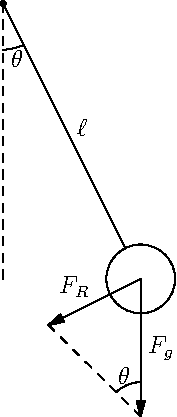
\includegraphics{images/pendulum.pdf}
 \caption{Pendulum!}
 \label{fig:pendulum}
\end{figure}
There is one missing force, $F_T$ or the the force due to the tension in the rod. Due to physics,
the sum of the forces on the mass should be 0. The only forces on the mass are $F_T$ and $F_R$,
the torque and restoring force. Therefore, our differential equation is given by,
\[
 m\ell\frac{d^2\theta}{dt} + mg\sin(\theta) = 0.
\]
Or, for simplification,
\[
 \frac{d^2\theta}{dt} = -\frac{g}{\ell}\sin(\theta).
\]
We'll assume $g=10$ and $\ell=1$.

Use the Runge-Kutta method to solve this system for $0\le t\le 10$ and the following initial conditions,
\begin{enumerate}
 \item $\theta_0 = \frac{\pi}{3}$, $\frac{d\theta}{dt}|_{t=0} = 0$
 \item $\theta_0 = \frac{\pi}{2}$, $\frac{d\theta}{dt}|_{t=0} = 0$
 \item $\theta_0 = 0$, $\frac{d\theta}{dt}|_{t=0} = \frac{\pi}{2}$
 \item $\theta_0 = \pi$, $\frac{d\theta}{dt}|_{t=0} = 0$
\end{enumerate}
For each initial condition, make the following graphs,
\begin{enumerate}
 \item A plot of $\theta$ vs $t$
 \item A plot of $y$ vs $x$, the position of the pendulum. Make sure the boundaries of this graph
are a square with side length 2.2, otherwise the motion won't look right.
\end{enumerate}

Describe what you see in each graph and briefly why it's happening.

\end{problem}




%Simple Pendulum


%Bioinforamtics stuff?


\end{document}






























